% preamble and style file for M&R lecture slides
\documentclass[11.5pt,sans,english]{beamer}

\usetheme{EastLansing}
\usecolortheme{lily}

\usepackage[most]{tcolorbox}

\usepackage{verbatim}
%\usepackage{ulem}
%\usepackage{fontawesome}
%\usepackage{tikz}
%\usepackage{pifont}
%\usepackage{tabularx}
\usepackage{array,booktabs,xcolor,colortbl,multirow,rotating,amssymb}
%\usepackage{amsmath}
% \usepackage{vwcol}
% \usepackage[T1]{fontenc}

  
\newcommand\vect[1]{\underline{\mathbf{#1}}}
\newcommand\unitvect[1]{\hat{\boldsymbol{#1}}}
%\newcommand\hatdot[1] { \hat{ \dot{ \boldsymbol{#1} } } }

\newtcbox
{\keyc}{on line,arc=2pt, colback=yellow!30!white, colframe=yellow!30!black, before upper={\rule[-3pt]{0pt}{10pt} },boxrule=1pt,boxsep=0pt,left=6pt,right=6pt,top=2pt,bottom=2pt,}

\newtcbox
{\keyb}{on line,arc=1pt, colback=blue!30!white, colframe=blue!30!black, before upper={\rule[-3pt]{0pt}{10pt} },boxrule=1pt,boxsep=0pt,left=6pt,right=6pt,top=2pt,bottom=2pt,}

\newtcbox
{\keyl}{on line,arc=1pt, colback=pink!30!white, colframe=blue!30!black, before upper={\rule[-3pt]{0pt}{10pt} },boxrule=1pt,boxsep=0pt,left=6pt,right=6pt,top=2pt,bottom=2pt,}

\newtcbox
{\keyw}{on line,arc=1pt, colback=red!30!white, colframe=blue!30!black, before upper={\rule[-3pt]{0pt}{10pt} },boxrule=1pt,boxsep=0pt,left=6pt,right=6pt,top=2pt,bottom=2pt,}

\newtcbox
{\keya}{on line,arc=1pt, colback=purple!30!white, colframe=blue!30!black, before upper={\rule[-3pt]{0pt}{10pt} },boxrule=1pt,boxsep=0pt,left=6pt,right=6pt,top=2pt,bottom=2pt,}

\newtcbox[auto counter,number within=section]
{keyf}
{
enhanced,
on line,
  boxsep=0pt,
  left=6pt,right=6pt,top=2pt,bottom=2pt,
  arc=5pt,
  boxrule=1pt,
  rightrule=38pt,
colback=green!10!white, 
colframe=green!50!black, 
title=\thetcbcounter,
detach title,
overlay unbroken and first ={
    \node[%rotate=90,
          %minimum width=1cm,
          anchor=south,
          font=\sffamily\bfseries\tiny,
          %yshift=-10pt,
          yshift=-5pt,
          xshift=-20pt,
          white]
    at (frame.east) {\thetcbcounter};
  }
}


\usepackage{xcolor}

%\usepackage{hyperref}
%\hypersetup{
%  pdfauthor={Lily Asquith},
%  urlcolor=blue,
%  colorlinks=true,
%  linkcolor=blue,
%  bookmarks=true
%}

%---------------------------------------------%
%              LILY'S COLOURS           %
%---------------------------------------------%
\definecolor{Wash}{RGB}{204,204,204}
%\definecolor{Pinky}{RGB}{254,200,254}%violet
\definecolor{Pinky}{RGB}{219,	240,	253}%violet
\definecolor{Bluey}{RGB}{0,190,255}%deep sky blue
\definecolor{DarkGrey}{RGB}{28,66,137}%dar grey
\definecolor{SussexWhite}{RGB}{253,255,254}%dar grey
\definecolor{LightGray}{RGB}{184,184,255}
\definecolor{YesGreen}{RGB}{0,128,0}
\definecolor{NoRed}{RGB}{250,0,0}



\definecolor{myred}{RGB}{255,153,153}
\definecolor{myorange}{RGB}{255,204,153}
\definecolor{myyellow}{RGB}{255,255,153}
\definecolor{mygreen}{RGB}{153,255,153}
\definecolor{mycyan}{RGB}{153,255,255}
\definecolor{myblue}{RGB}{153,204,255}
\definecolor{myviolet}{RGB}{153,153,255}
\definecolor{mypurple}{RGB}{204,153,255}
\definecolor{mypink}{RGB}{255,204,255}
\definecolor{mycoral}{RGB}{255,153,204}

%-----------------------------------------------------%
%              LILY'S COLUMN TYPES          %
%-----------------------------------------------------%
\newcolumntype{a}{>{\raggedright\arraybackslash}l}	
\newcolumntype{q}{>{\raggedright\arraybackslash}m{8cm}} 

%--------------------------------------------%
%              LILY'S SYMBOLS          %
%--------------------------------------------%
\newcommand{\dfinger}{\large{\textcolor{black}{\ding{43}}}\scriptsize}
\newcommand{\dstar}{\large{\textcolor{black}{\ding{76}}}\scriptsize}
\newcommand{\dwrite}{\large{\textcolor{black}{\ding{45}}}\scriptsize}
\newcommand{\ddiamond}{\small{\textcolor{DarkGrey}{\ding{117}}}\scriptsize}
\newcommand{\ddiamondwhite}{\small{\textcolor{SussexWhite}{\ding{117}}}\scriptsize}
\newcommand{\experiment}{\small{\textcolor{magenta}{\faCogs }}\scriptsize}
\newcommand{\watchit}{\textcolor{blue}{ \faYoutube}}


\makeatletter
\newcommand\notsotiny{\@setfontsize\notsotiny{6.5}{7.5}}
\makeatother


% 
\title[ Mechanics \& Relativity]{Mechanics \& Relativity}
\author[Dr Lily Asquith (Lily)]{ Dr Lily Asquith (Lily)}
\date[28-30 September 2021]{28-30 September 2021 (Week 1)}
\logo{

\includegraphics[width=1.5cm]{../../utils/uslogo.jpg}
}


\begin{document}


\begin{frame}
\titlepage
\end{frame} 

 %-----------------------------------------------------------%
 % 1 Kinematics                                                 %
 %-----------------------------------------------------------%
\section{M\&R 1: Kinematics}
\begin{frame}
\frametitle{Kinematics} 
\normalsize

This week's topics:\\[3ex]

\begin{itemize}
\item[1.1] Displacement, Velocity \& Acceleration\\[3ex]
\item[1.2] Equations of motion (SUVAT)\\[3ex]
\item[1.3] Reading graphs\\[3ex]
\end{itemize}
\end{frame} 
 
\begin{frame}{Quiz 1.2 suvat}
TBD
%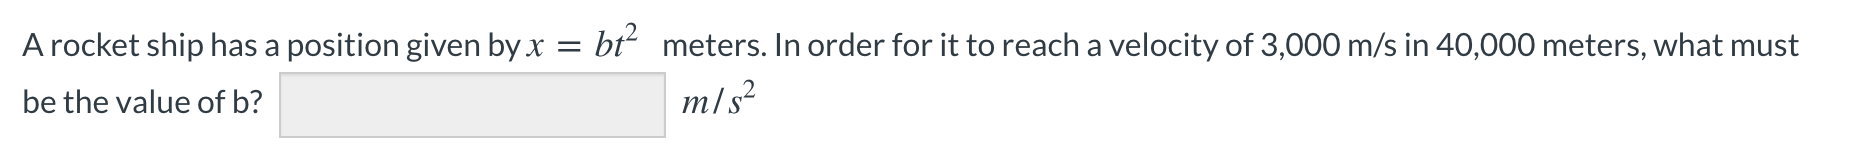
\includegraphics[scale=0.35]{rocket_question}
\vspace{6cm}
\end{frame}




\begin{frame}{Poll Everywhere Checkpoint}

You are standing on a bridge with two eggs. You drop one, and you throw the other directly downwards.\\

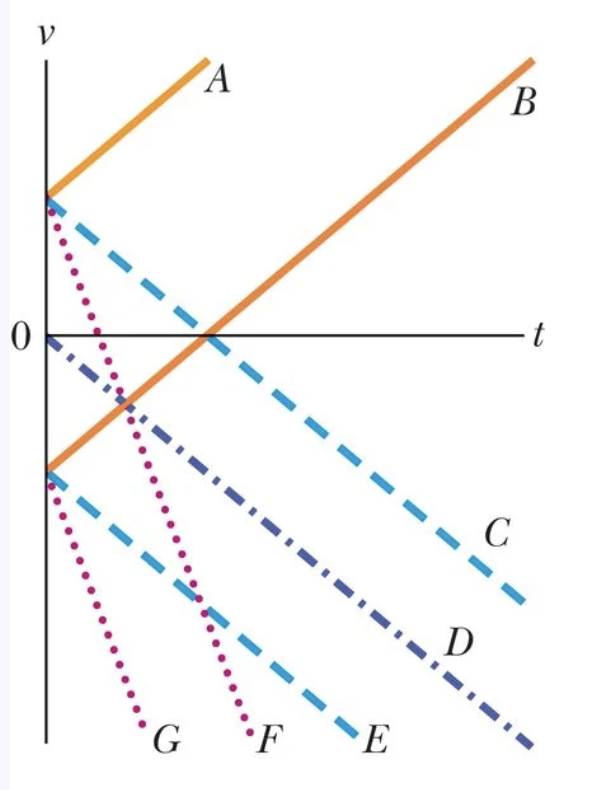
\includegraphics[scale=0.3]{vt-graph}
 
\fbox{\begin{minipage}{\textwidth}
Use your phone to go to: \textcolor{blue}{pollev.com/ilovephysics}\\
 (a) Which line best describes the motion of the dropped egg? \\
 (b) Which line best describes the motion of the thrown egg?\\
\end{minipage}}
\vspace{2cm}

\end{frame}

%-----------------------------------------------------
%     LECTURE 3
%-----------------------------------------------------

\subsection{Reading graphs }


\begin{frame}{Integrating acceleration over time}
\small
We know that $a = \frac{dv}{dt}$\\

\begin{equation}\nonumber
\begin{split}
\displaystyle \int_{t_0}^{t} a dt  & = \displaystyle\int_{t_0}^{t} \frac{dv}{dt} dt\\
  & = \displaystyle \int_{t_0}^{t} dv \\
  & = v_{t} - v_{t0} \\
\end{split}
\end{equation}

\keyf{$ \displaystyle \int_{t_0}^{t} a dt   = v_{t} - v_{t0} $ }  \keyc{The integral of the acceleration over time gives the change in velocity}\\[1ex]



\end{frame}


\begin{frame}{Integrating velocity over time}
\small
Similarly $v = \frac{ds}{dt}$\\

\begin{equation}\nonumber
\begin{split}
\displaystyle \int_{t_0}^{t} v dt  & = \displaystyle\int_{t_0}^{t} \frac{ds}{dt} dt\\
  & = \displaystyle \int_{t_0}^{t} ds \\
  & = s_{t} - s_{t0} \\
\end{split}
\end{equation}

\keyf{$ \displaystyle \int_{t_0}^{t} v dt   = s_{t} - s_{t0} $ }  \keyc{The integral of the velocity over time gives the change in position}\\[1ex]

\end{frame}

\begin{frame}{The area under a curve}
\notsotiny
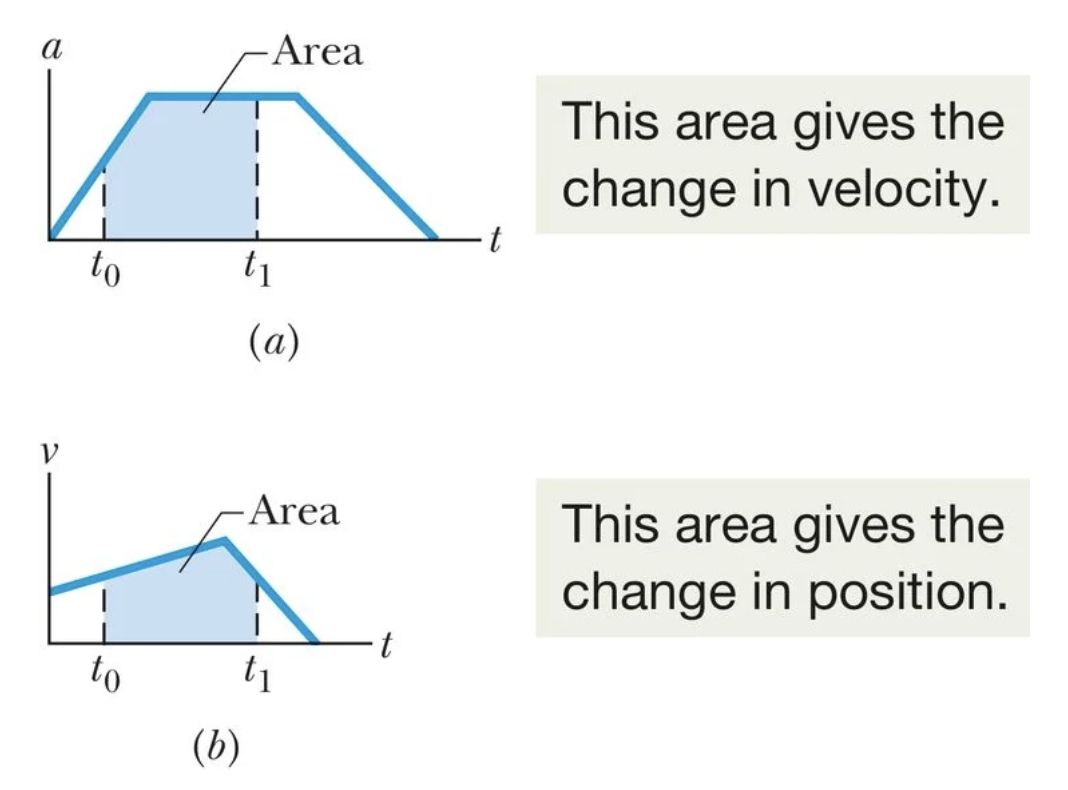
\includegraphics[scale=0.3]{area-under-curve}
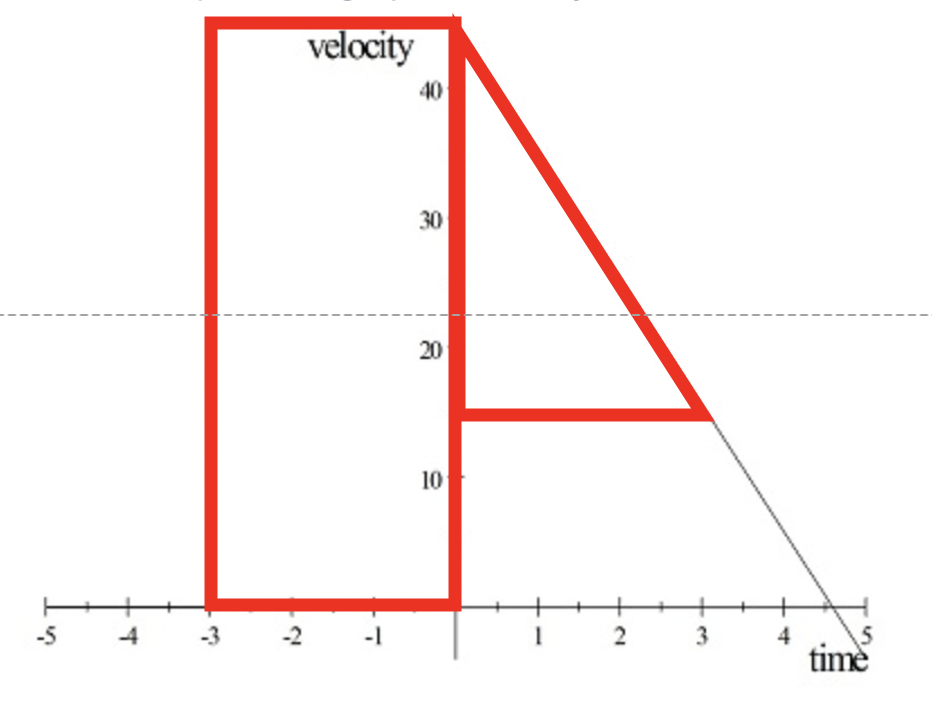
\includegraphics[scale=0.3]{area-under-curve-2}
\end{frame}


\begin{frame}{A example: whiplash curve}
\notsotiny
%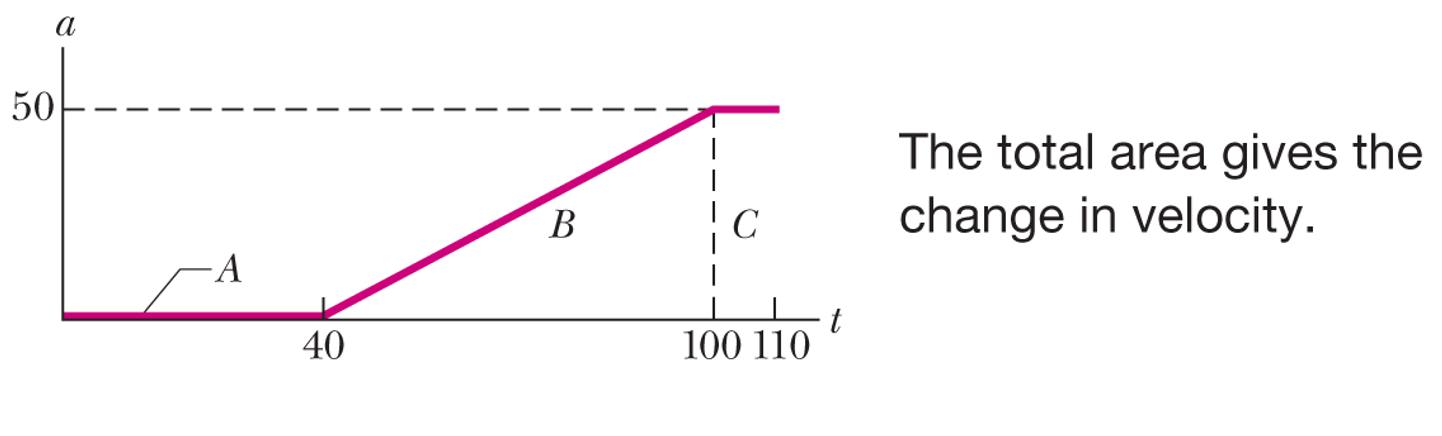
\includegraphics[scale=0.3]{whiplash1}

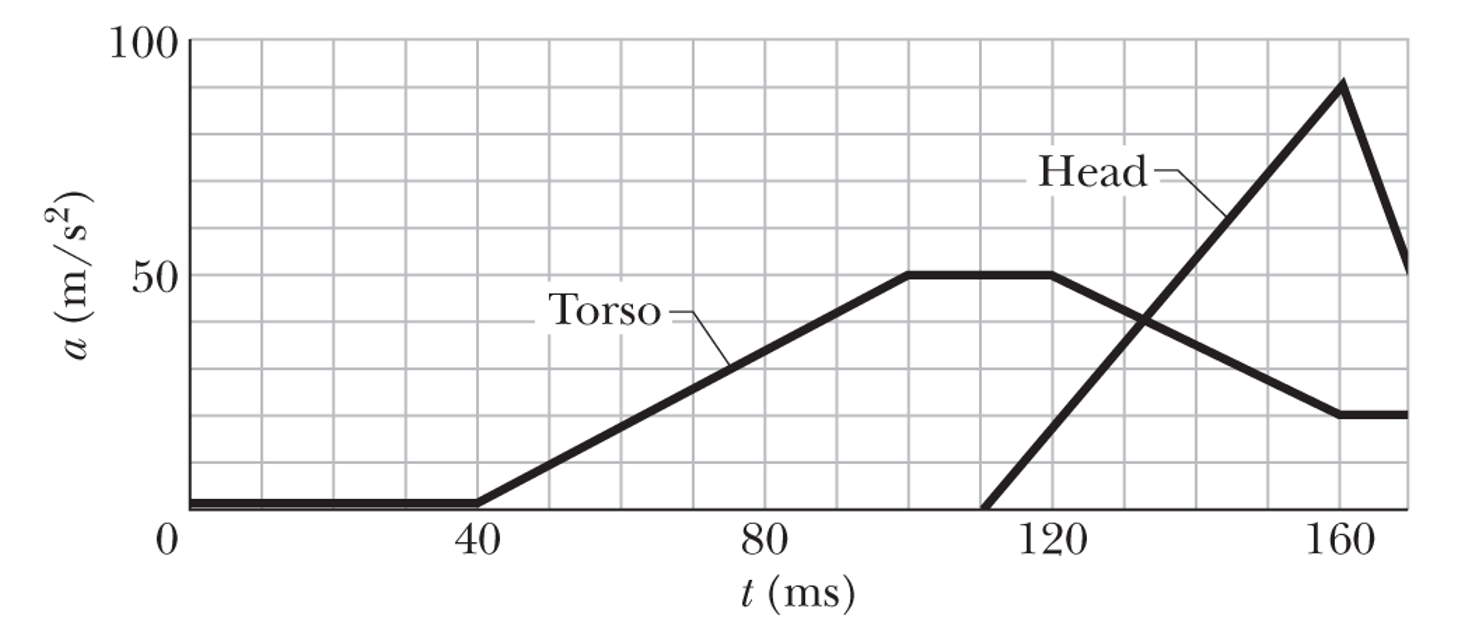
\includegraphics[scale=0.3]{whiplash2}
\end{frame}



\begin{frame}{Tackling confusion with directions}
\notsotiny
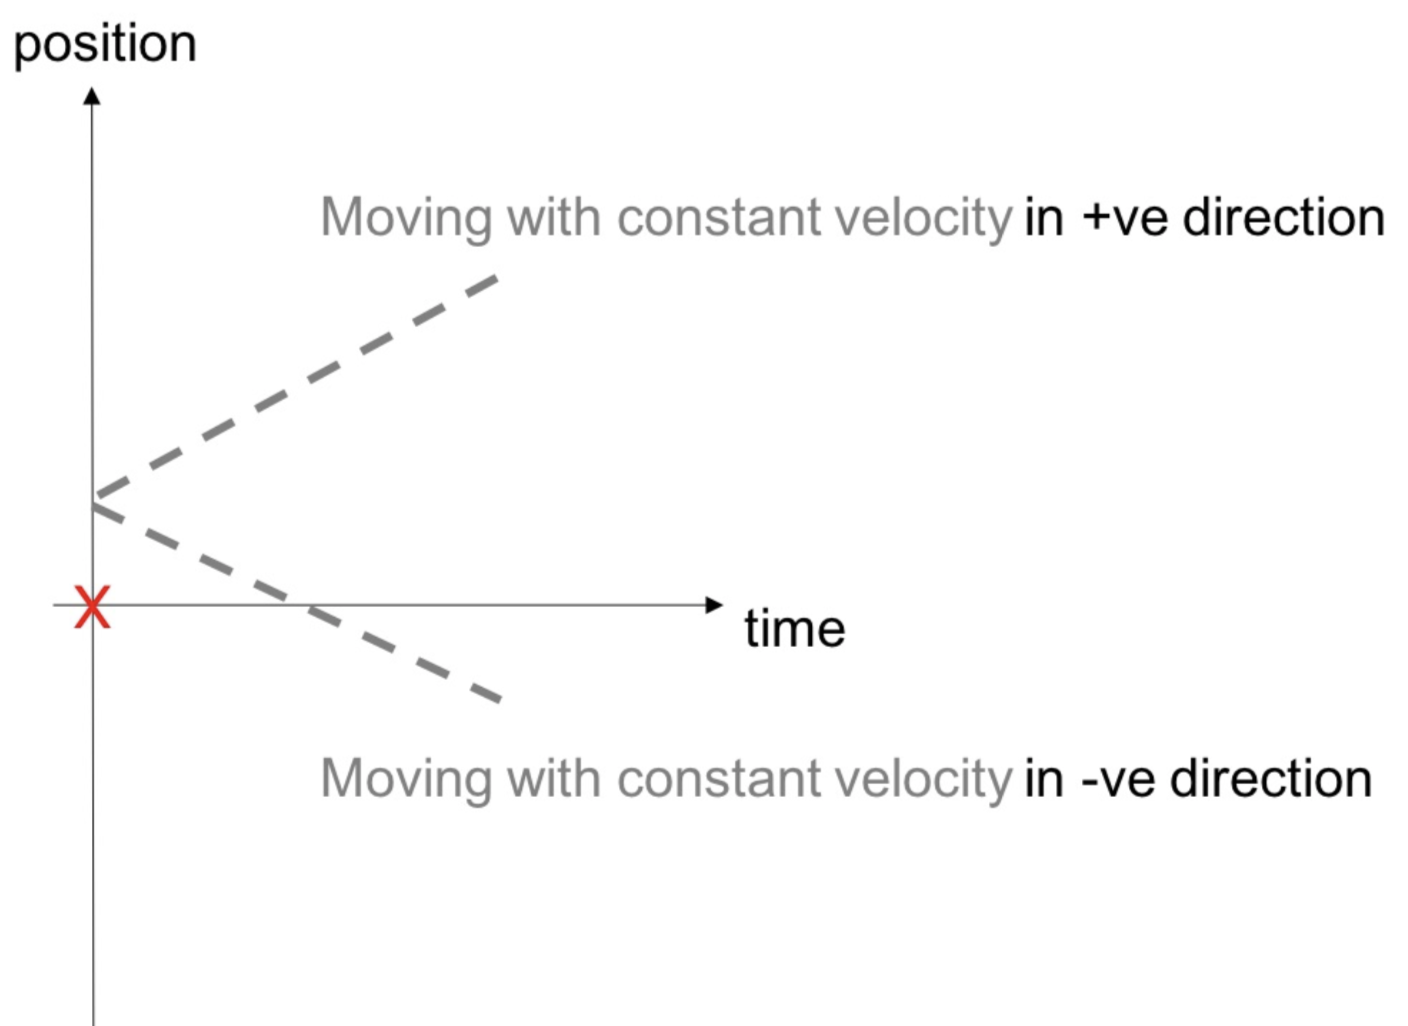
\includegraphics[scale=0.3]{PositionTime}

\end{frame}

\begin{frame}{Zero velocity is constant velocity}
\notsotiny
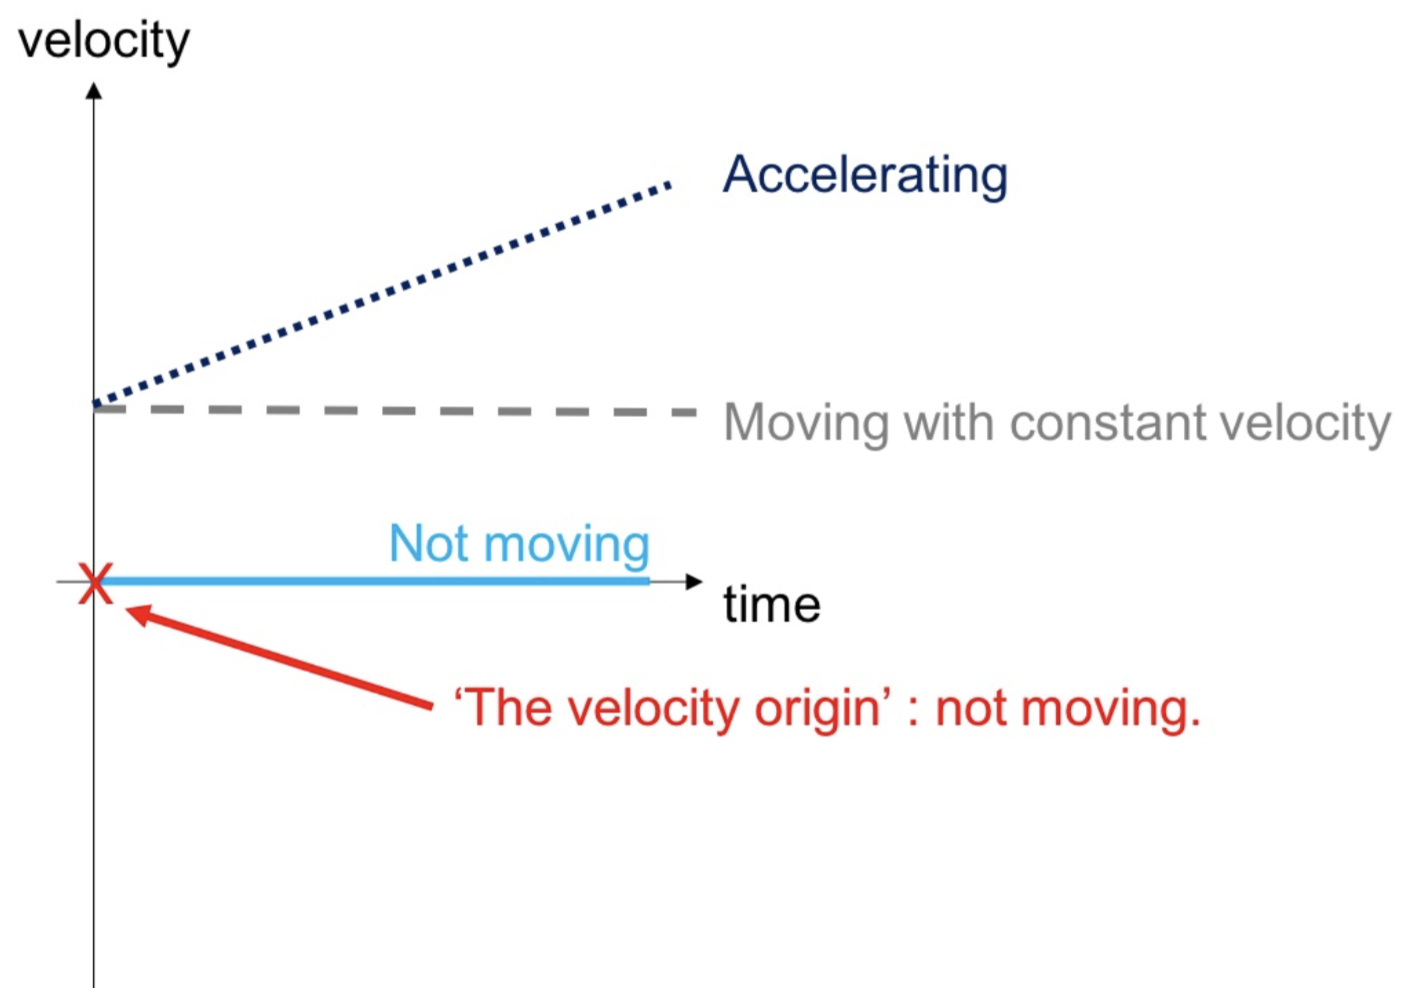
\includegraphics[scale=0.3]{VelocityTime}

\end{frame}


\begin{frame}{Matching slopes to values}
\notsotiny
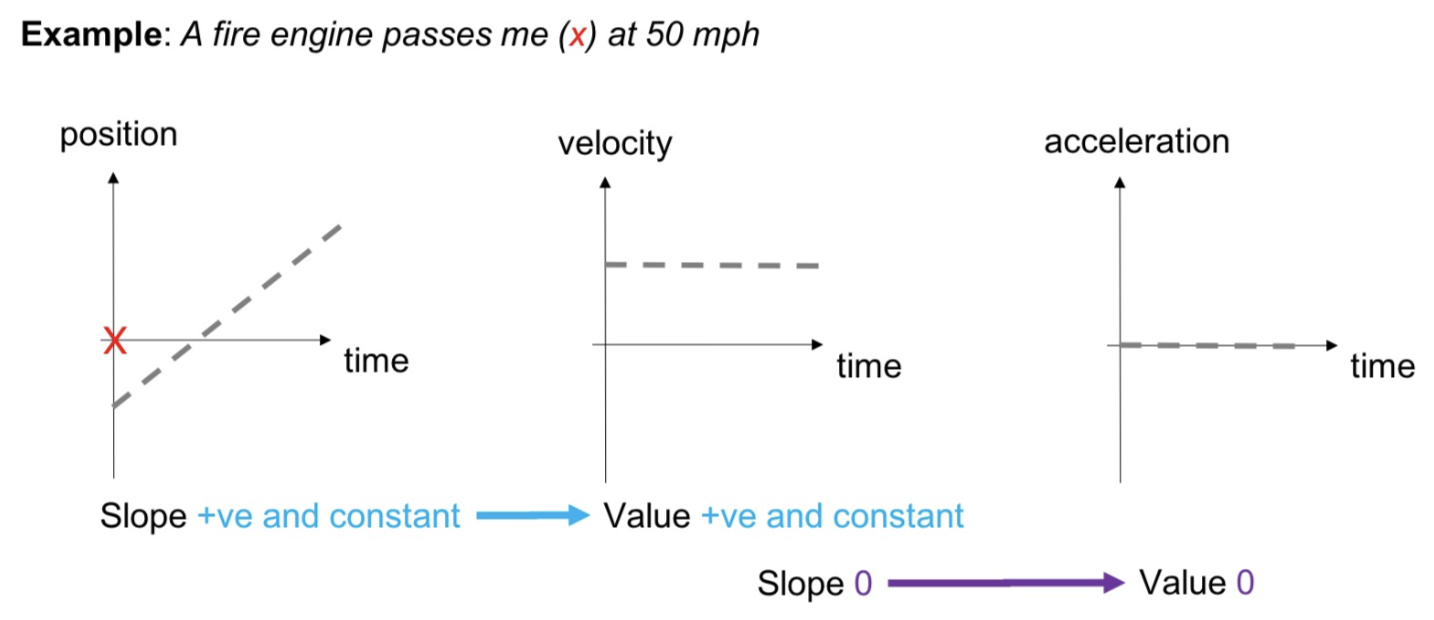
\includegraphics[scale=0.4]{FireEngine}

\end{frame}


\begin{frame}{A bouncing ball}
\small
How would we draw the motion of a ball being dropped from height, reaching ground, and bouncing back up again?\\
\vspace{5cm}

\end{frame}


\begin{frame}{Divide \& Conquer}
\notsotiny
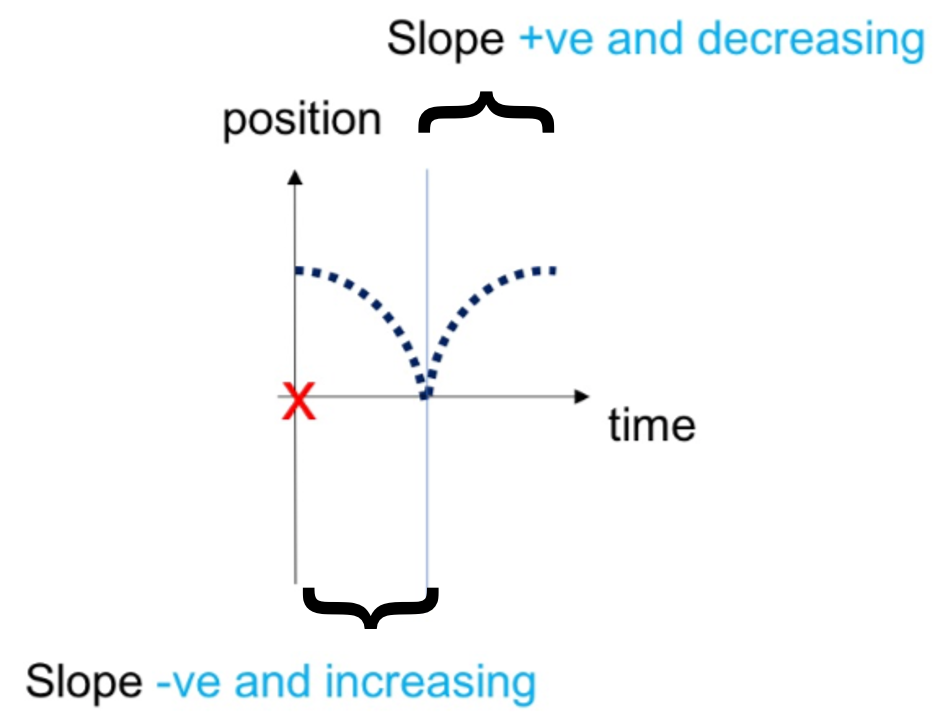
\includegraphics[scale=0.4]{ball1}

\end{frame}

\begin{frame}{Divide \& Conquer}
\notsotiny
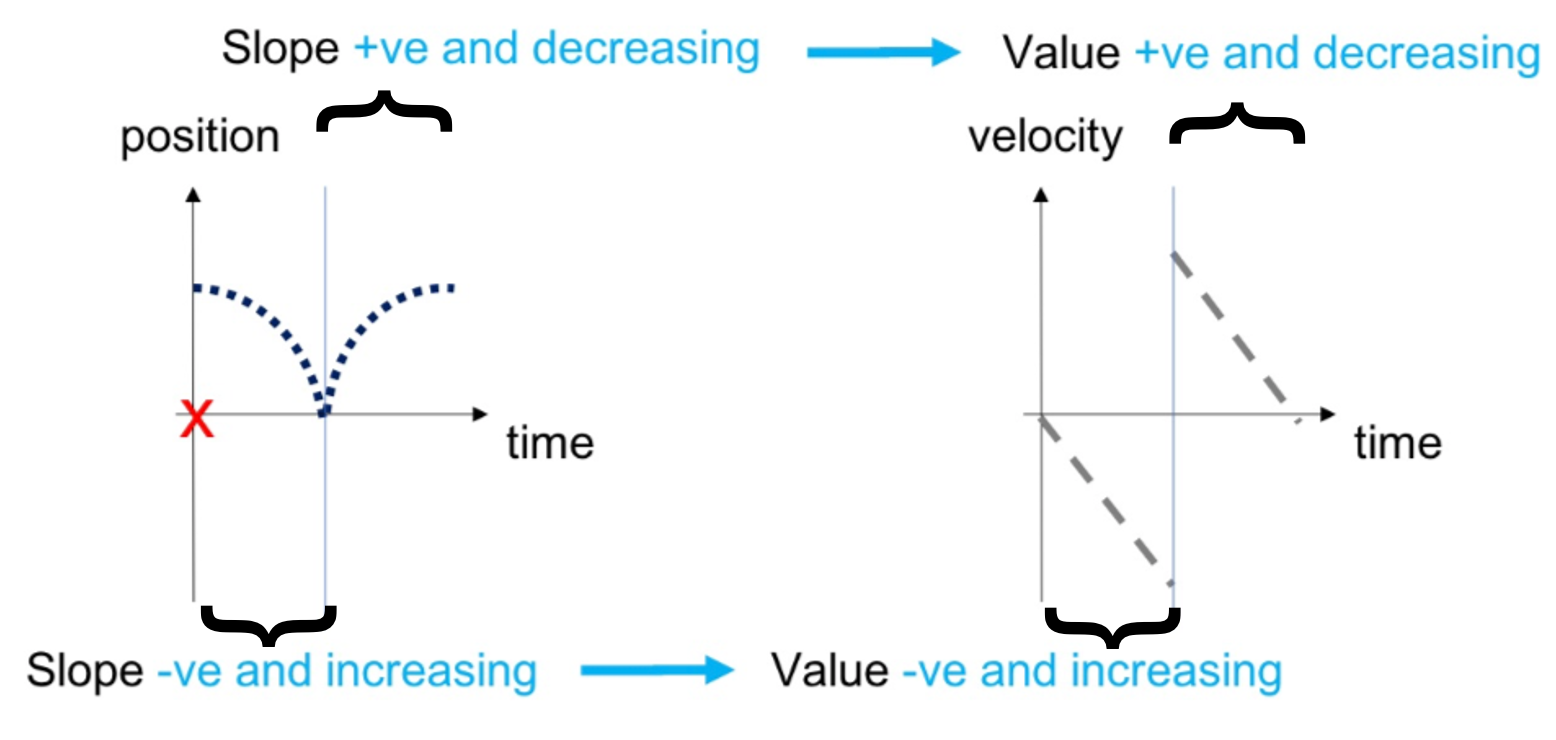
\includegraphics[scale=0.4]{ball2}

\end{frame}

\begin{frame}{Divide \& Conquer}
\notsotiny
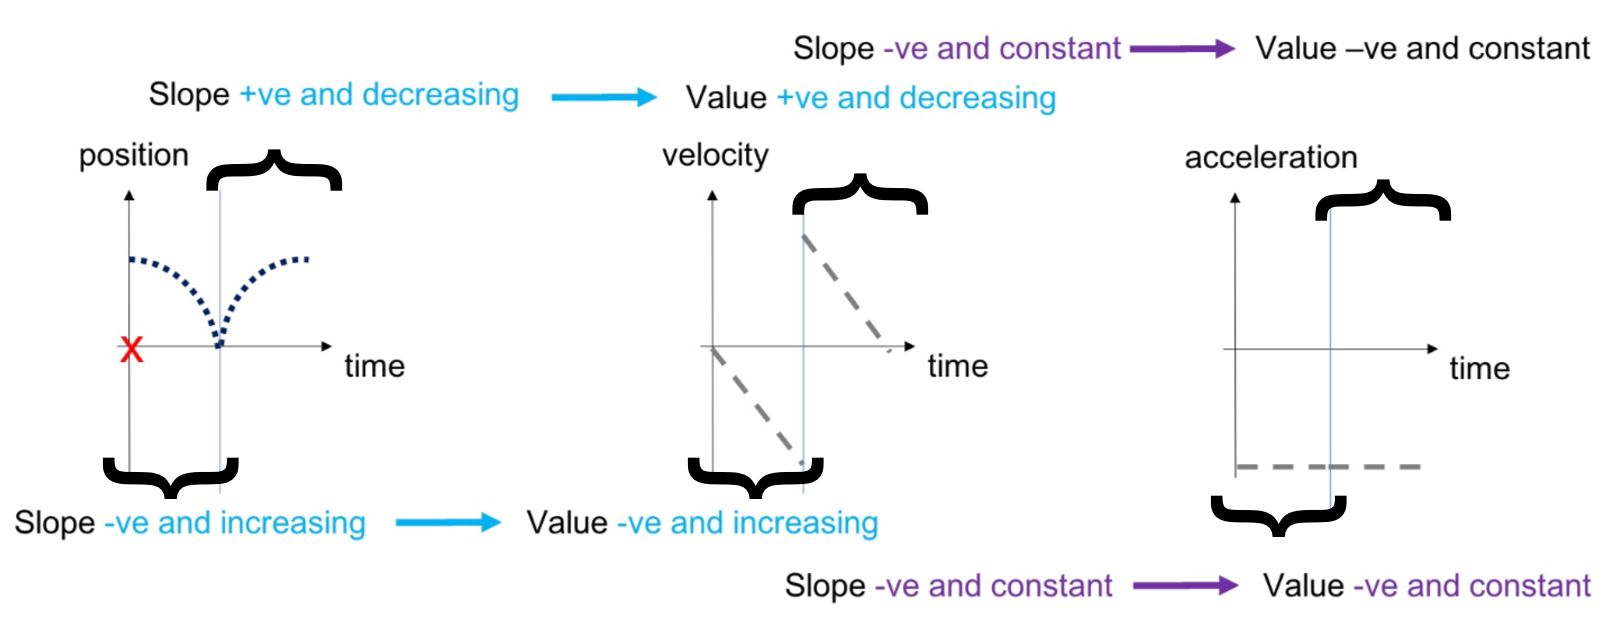
\includegraphics[scale=0.4]{ball3}

\end{frame}

\begin{frame}{Poll Everywhere Checkpoint (\textcolor{blue}{pollev.com/ilovephysics})}
\notsotiny
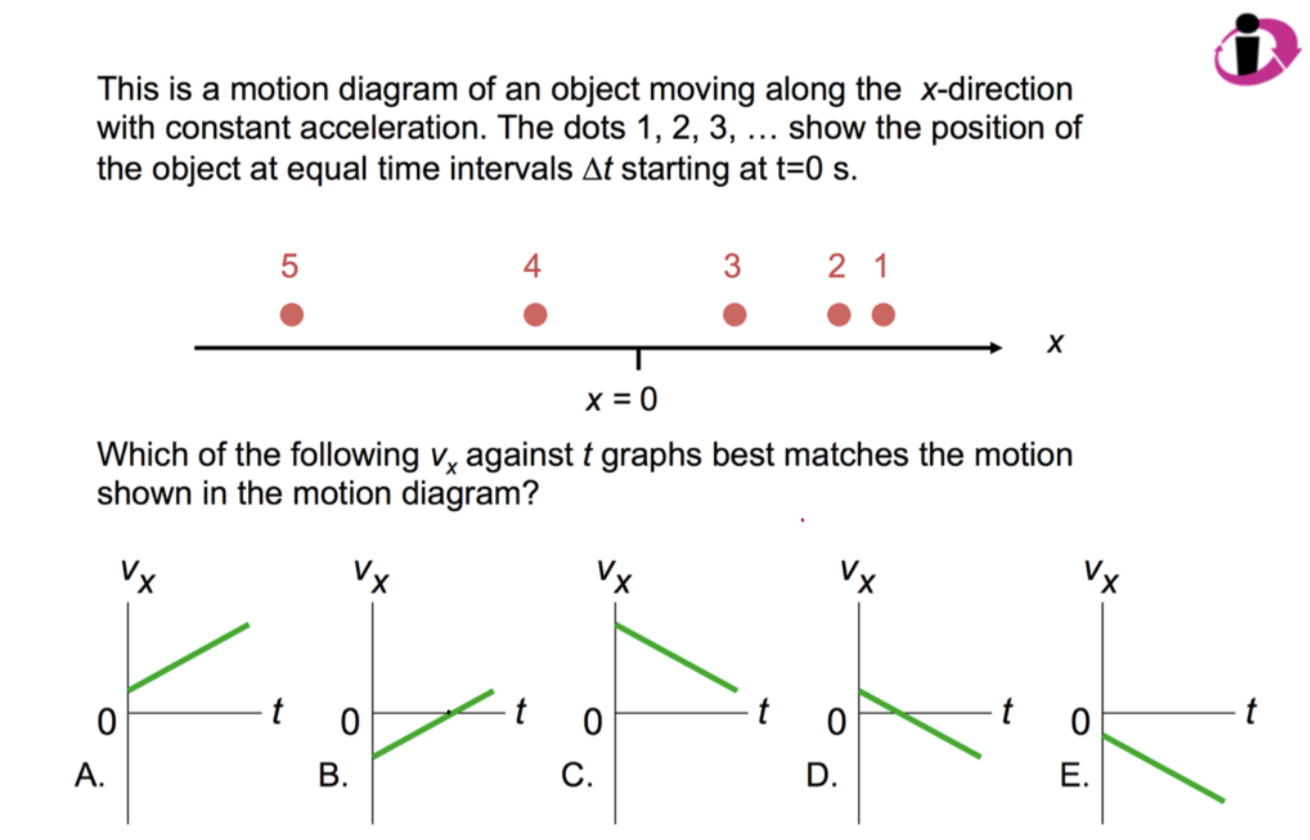
\includegraphics[scale=0.4]{GraphQuiz}

\end{frame}

\begin{frame}{Reading graphs: additional problem}
\notsotiny
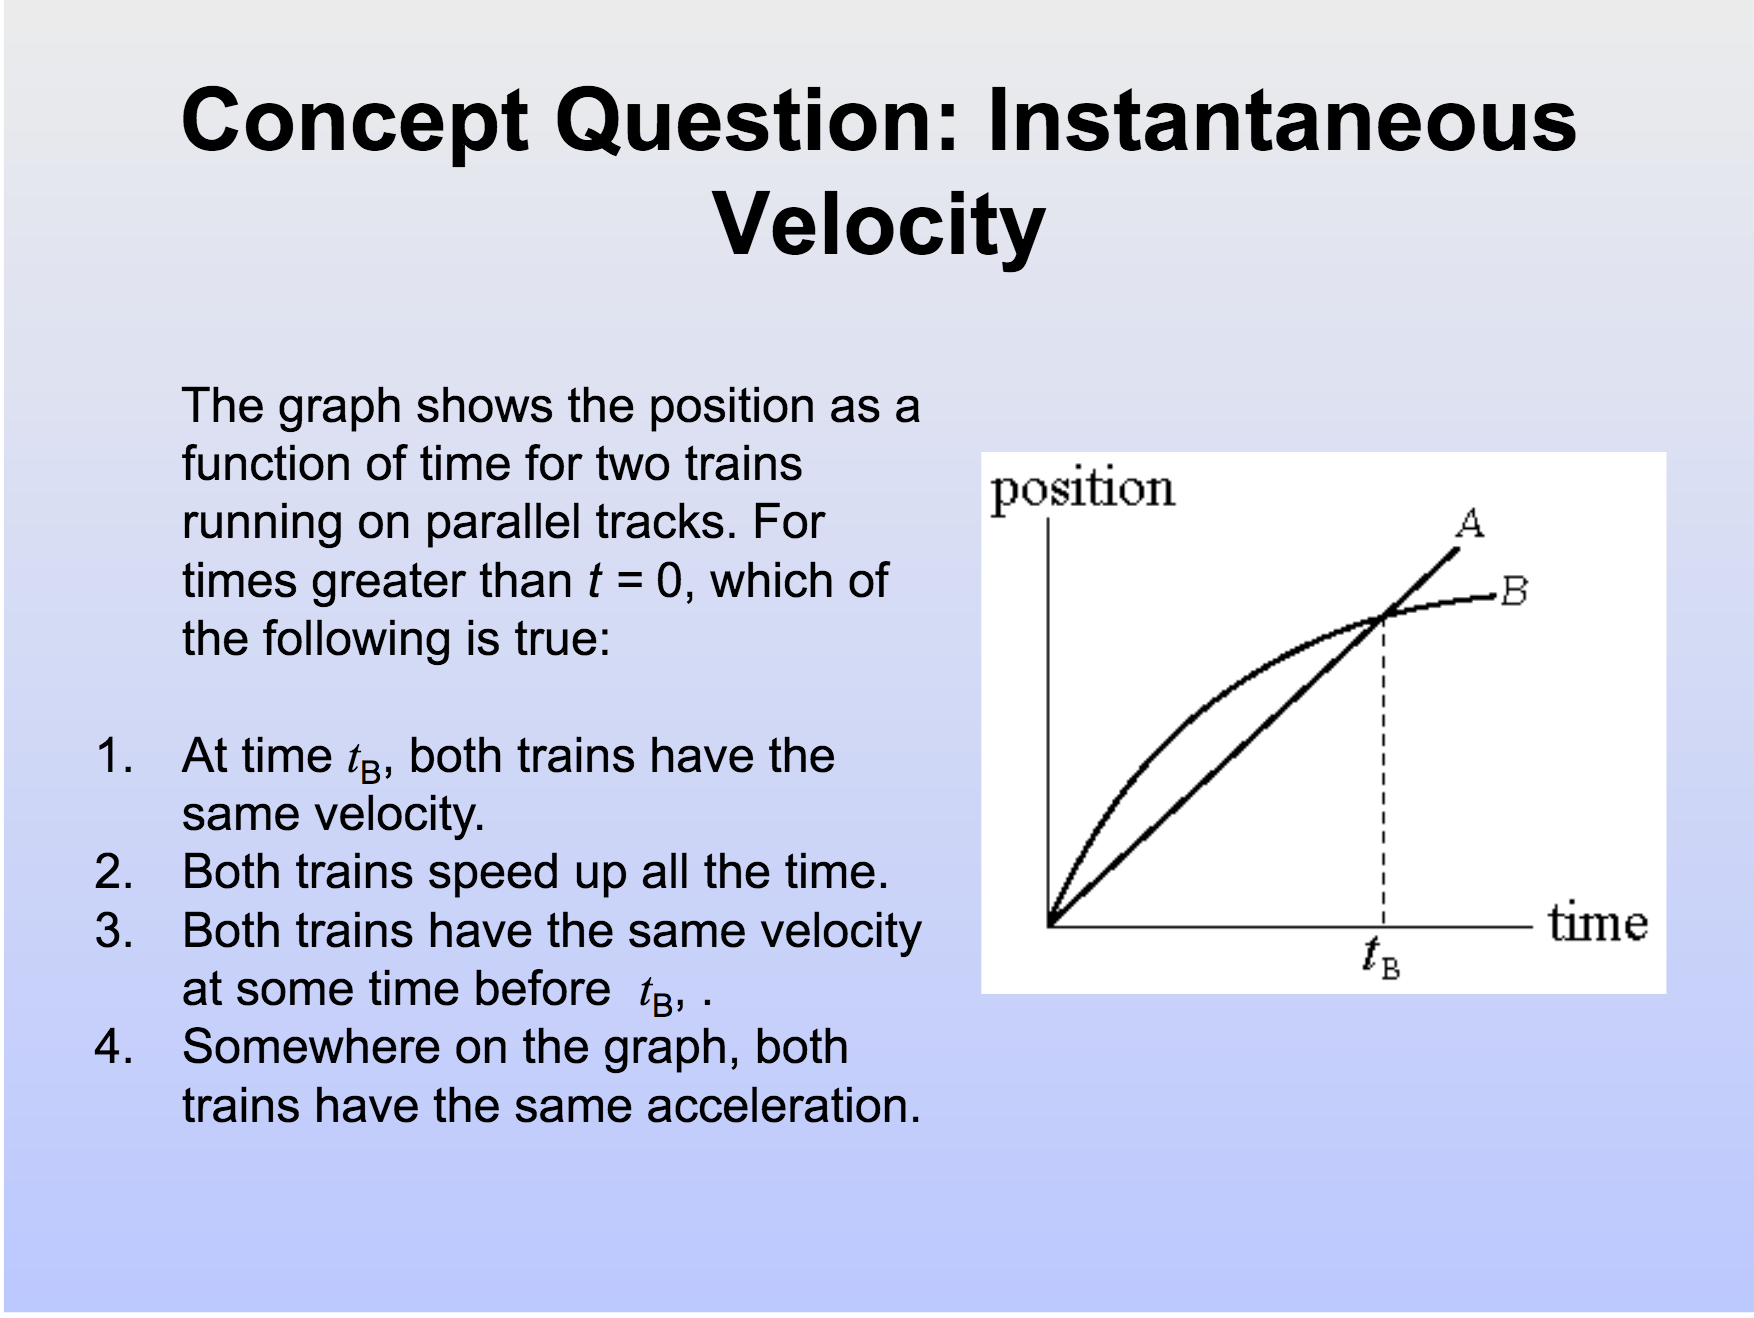
\includegraphics[scale=0.3]{NickedFromMIT}

\end{frame}



\begin{frame}{Preparing for next week's Kinematics Workshop}
\small
\begin{itemize}
\item The problems for the workshop are on Canvas.
\item Have a go at the problems prior to your workshop, so you know in advance what you would like the DT's help with.
\item Each workshop has a question marked out as the one you will be graded on.
\item Upload your solution to this before the end of next week.
\end{itemize}
\end{frame}

\begin{frame}{Tips}
\small
\begin{itemize}
\item You will need to use the quadratic formula at least once, so remind yourself what that is and when it is useful.
\item What information is given in the question? Write it down.
\item What information is known but not given? Write it down.
\item Underline or draw a box around your answer and take a photo of it (including working) and upload it to canvas.
\end{itemize}
\end{frame}
 
\end{document}